\chapter{PID Controller Considerations}
\label{chap:PIDControllerConsideration}
\abstract{In this chapter the metrics used for performance and robustness evaluation are presented for the case of \gls{pid} control. Special attention is given to the integral measure of error as well as the trade-offs that arise in a controlled system. For example, the well-known relationship between servo and regulation response, or between performance and robustness. These trade-offs are what gives meaning to the multiobjective approach that will be presented in the rest of the book.}

\section{Control System Evaluation Metrics}
%
Needless to say, specific design criteria is important in order to have a quantitative metric of the usefulness of controller tuning. However, it becomes an indispensable tool when combining different control system specifications, as it happens in a multiobjective approach.

It has been common practice in control systems literature to use different indexes to measure the accomplishment of such specifications, both from the point of view of performance as well as robustness.

Taking into account that in industrial process control applications a good load-disturbance rejection along with a good transient response to set-point changes is required, the controller design should consider both possibilities of operation. Despite this, the servo and regulation demands cannot be optimally satisfied simultaneously with a \gls{1dof} controller, because the resulting dynamic for each operation mode is different and only one optimal solution can be chosen. Therefore, there will be the need to quantify the level of \emph{performance} accomplishment regarding each one of the operational modes.

On the other hand, the control system design is usually based on the use of low-order linear models; these models in turn are based on the normal operating point of the closed-loop control system. Because most industrial processes are non-linear, it is necessary to account for possible changes in the process characteristics by adopting certain relative stability margins or \emph{robustness} requirements for the control system.

Therefore, in the design of a closed-loop control system with \gls{pi} and \gls{pid} controllers, we must consider the trade-off between two conflicting criteria: the time-response performance to the set point and load disturbances and the robustness to changes in the characteristics of the controlled process. In order to manage those conflicting objectives, suitable metrics are presented in what follows.
 
\subsection{Performance}
%
The performance of a control system may be evaluated by using different measures. In control textbooks it is usual to find a characterization of the time response in terms of numerical quantities assimilated to a second-order under-damped system such as: percentage overshoot, rise time, etc. However, in academic and research works it is more common and convenient to use a cost function based on the error, i.e. the difference between the desired value (set-point) and the actual value of the controlled variable (system's output).  Of course, as larger and longer in time is the error, the system's performance will be worse. In recent years those cost functions related to the integrated error have become very popular, given by the following general formulation:
%
\begin{equation}
	J_{e} \doteq \int^{\infty}_{0} t^p \left|e(t)\right|^q dt,  \label{eq:generic_index}
\end{equation}
%
where the error can be generated because either a set-point changes or a load-disturbance appears.

A review of research history on \gls{pid} controller design reveals that, among the most used ones, there have been the \gls{iae}, the \gls{itae}, or the \gls{ise}. From an academic point of view, objective functions can take any one wished form. However, from an industrial point of view, realistic economic objectives need to be addressed. As it is desirable to use a performance indicator that takes into account economic considerations, the \gls{iae} is suggested by \citet{Shinskey2002} as a meaningful measure since it can be assimilated to product giveaway, excess consumption of utilities, and reduction in plant capacity. Taking this into account, to avoid the cancellation of positive and negative errors, there seems to be a \emph{de facto} agreement with the use of the \gls{iae}, $p=0$, $q=1$ in \eqref{eq:generic_index}, given by:
%
\begin{equation}
	J_e \doteq \int^{\infty}_{0} \left|e(t) \right| dt = \int^{\infty}_{0} \left|r(t)-y(t) \right| dt. 
\end{equation}
%
%----------------------------------------------------
%
\subsection{Robustness}
%
Robustness is an important attribute for control systems, because the design procedures are usually based on the use of low-order linear models identified at the closed-loop operation point. Due to the non-linearity found in most industrial processes, it is necessary to consider the expected changes in the process characteristics by assuming certain relative stability margins, or robustness requirements, for the control system.

The robustness is a measure of how much change the controller can tolerate in the process transfer function; more specifically, in its gain and in its phase lag.

In this case, there are some useful indicators that can be implemented as design criteria for robustness. The most widely accepted in industrial practice are the gain and phase margin. The \emph{gain margin $A_m$} is a measure of how much the process gain can change before the closed loop system becomes unstable. Control theory states it is the amount of gain increase or decrease required to make the loop gain unity at the frequency where the phase angle is $-180^\circ$. Therefore leading the closed-loop system to the critical point. On the other hand, the \emph{phase margin $\phi_m$} is a measure of how much the process phase can change before the closed-loop system becomes unstable. The phase could be increased because of an additional delay or because the process lag decreased.

The use of the gain and phase margins as robustness measures has been replaced by the use of a single indicator: the maximum of the sensitivity function, denoted by $M_s$, defined by the shortest distance from the Nyquist diagram to the real point $-1$; this maximum sensitivity is strictly related to the gain and phase margin through some simple inequalities. Then, for each controller parameter set obtained, the closed-loop control system robustness is measured using the control system Maximum Sensitivity $M_s$ defined as:
%
\begin{equation}
M_{s} \dot{=} \max_{\omega} \left|S(j \omega)\right| = \max_{\omega} \frac{1}{\left|1+C(j \omega) P(j \omega)\right|}.
\label{Eq:Ms}
\end{equation}

The recommended values for $M_s$ are typically within the range 1.4 - 2.0. For a particular value of $M_s$, the lower bounds to the gain margin $A_m$, and phase margin $\phi_m$, are given by \citep{astromhagglund2006}:
%
\begin{eqnarray*}
    A_m > \frac{M_s}{M_s-1} \quad ; \quad \phi_m > 2 \sin^{-1} \left(\frac{1}{2 M_s} \right)
\end{eqnarray*}

Therefore, ensuring $M_s=2.0$ provides what is commonly considered minimum robustness requirement (that translates to $A_m> 2$ and $\phi_m > 29^\circ$, for $M_s=1.4$  we have $A_m > 3.5$ and $\phi_m > 41^o$). Even if there are different measures for the closed-loop system robustness, $M_s$ is widely used as a reasonable robustness measure.
%
%\centerline{\textcolor{red}{TAKE A LOOK AT THE MODULUS MARGIN}}
%
\subsection{Control Input Usage}
%
Controller design problems are stated in terms of the controlled variable (usually the process output). Depending on how this problem is stated and solved, this may generate controller settings that produce command signals that are either undesirable or unrealistic. It is therefore always needed to evaluate the control signal and take care of the controller bandwidth. This is usually related to the variation of the control signal as a measure of its \emph{smoothness}. For the evaluation of the required \emph{control effort}, the control signal total variation ($TV_u$) is computed by the difference between the values of the control variable at two consecutive sampling time instants as:
%
\begin{equation}
	TV_u \doteq \sum^{\infty}_{k=1} \left|u_{k+1} - u_k \right|,  \label{eq:p02}
\end{equation}
%
and it is used as the main indicator of smoothness of the control action.

As a complementary measurement of the control effort, the controller output instantaneous change to a set-point step change (the ``proportional kick'', $\Delta u_0$) can be considered:
\begin{equation}
	\Delta u_0 \doteq \beta K_p \Delta r, \label{eq:p02du}
\end{equation}

\section{Control System Trade-offs}
%
As stated before, the performance of the controlled system can be measured using different cost functions. Some of these performance metrics are the set-point tracking, the disturbance rejection, the control effort reduction and the robustness.

It is well known that these goals cannot be achieved simultaneously \citep{Arrieta2010,alcantara2013}. In such case, a trade-off between the objectives is required. Improving one objective may yield to poor performance in another. As we have seen, every goal should be translated into design specifications, and specific indices in order to  measure the performance of the \gls{pid} controller.

Taking into account that in industrial process control applications, good load-disturbance rejection is required, as well as good transient response to set-point changes, the controller design should consider both possibilities of operation. Despite the above, the servo and regulation demands cannot be optimally satisfied simultaneously with a \gls{1dof} controller, because the resulting dynamic for each operation mode is different and it is possible to choose just one for an optimal solution. Considering the previous statement, most of the existing studies have focused only in fulfilling one of the two requirements, providing tuning methods that are optimal to servo-control or to regulation-control. However, it is well known that if we optimize the closed-loop transfer function for a step-response specification, the performance with respect to load-disturbance attenuation can be poor and vice-versa \citep{Arrieta2010a}. Therefore, it is desirable to get a compromise design, between servo/regulation when using \gls{1dof} controller.

Tuning is usually a compromise between performance and robustness. In fact, information about the process to be controlled takes the form of a model but this is always incomplete. Therefore, robustness is needed in order to preserve the basic properties that the model-based tuning provides. Among them, stability of the controlled system is a first need followed by the optimization of the performance. As a basic trade-off, as more robustness is imposed, the model-based tuning tends to provide lower performance. This is why some tunings focus exclusively on loop performance, whereas others are aimed to ensure robust stability, or a compromised mix of both. 

\subsection{Servo vs. Regulation}
%
%When tuning standard \gls{pid} controllers, it is hard to achieve good tracking and fast disturbance rejection at the same time. Given a particular tuning, if we want to improve disturbance rejection and get it faster, this requires more gain inside the bandwidth, which can only be achieved by increasing the slope near the crossover frequency. As a larger slope means getting closer to the critical (-1, 0j) point, this typically comes at the expense of more overshoot in response to set-point changes. Therefore worsening the set-point tracking. This is a frequency domain reasoning that is sometimes not familiar. Therefore, the use of time domain indexes like the ones presented above. A relatively low \gls{iae} corresponds to a relatively fast closed loop response and relatively low oscillatory behavior in the controlled variable (also represented by low values in the control effort measure). 
 
As we already know, the closed-loop transfer function between the set-point and the error signal is different from that of the load disturbance and error; therefore a low \gls{iae} in fast tracking task leads to slow-moving behavior with high \gls{iae} in the load disturbance rejection; conversely, a quick reaction to the disturbance means high overshoot in response to set-point step change, thus increasing its \gls{iae}. This is a well-known effect when zero-pole cancellation occurs in the closed-loop transfer function, which is a common practice for set-point tunings. It works well for the operation as a servo control system but since the closed-loop transfer function from the load disturbance to the error still contains the process modes, the regulation operation does not need to exhibit good performance measures.
 
It is common practice for \gls{1dof} controllers to relate the tuning method to the expected operation mode for the control system, \emph{servo} or \emph{regulation}. Therefore, controller settings can be found for optimal set-point or load-disturbance responses. This fact allows better performance of the controller when the control system operates on the selected tuned mode, but a degradation in the performance is expected when the tuning and operation modes are different. Obviously there is always the need to choose one of the two possible ways to tune the controller, for set-point tracking or load-disturbances rejection. In the case of \gls{1dof} \gls{pid}, tuning can be optimal just for one of the two operation modes.

In order to show how the performance of a system can be degraded when the controller is not operating according to the tuned mode, an example is provided. This motivates the analysis of the servo/regulation \emph{trade-off}.

Consider the following plant transfer function, taken from \citet{zhuang1993}, and the corresponding \gls{foptd} approximation:
%
\begin{equation}
P_1(s)=\frac{\me^{-0.5s}}{(s+1)^2} \approx \frac{\me^{-0.99s}}{1+1.65s}. \label{system_example} 
\end{equation}

\gls{pid} controller parameters are found in \citet{zhuang1993} by application of the \gls{ise} tuning formulae for optimal set-point and load-disturbance. Figure \ref{ch3:fig:example1} shows the performance of both settings when the control system is operating in both, servo and regulation mode. It can be observed that the load-disturbance response of the set-point tuning ($sp$) is closer to the optimal regulation one than the load-disturbance tuning ($ld$) to the optimal servo tuning. As a result, the observed performance degradation is larger for the load-disturbance tuning. A search for a compromise among both tunings is needed, and since only one has to be taken, it seems better to choose the set-point setting. However, in situations like this where there are conflicting objectives, a more complex approach is needed in order to find the best trade-off, according to the operator's aims.
%
\begin{figure}[tb]
    \begin{center}
        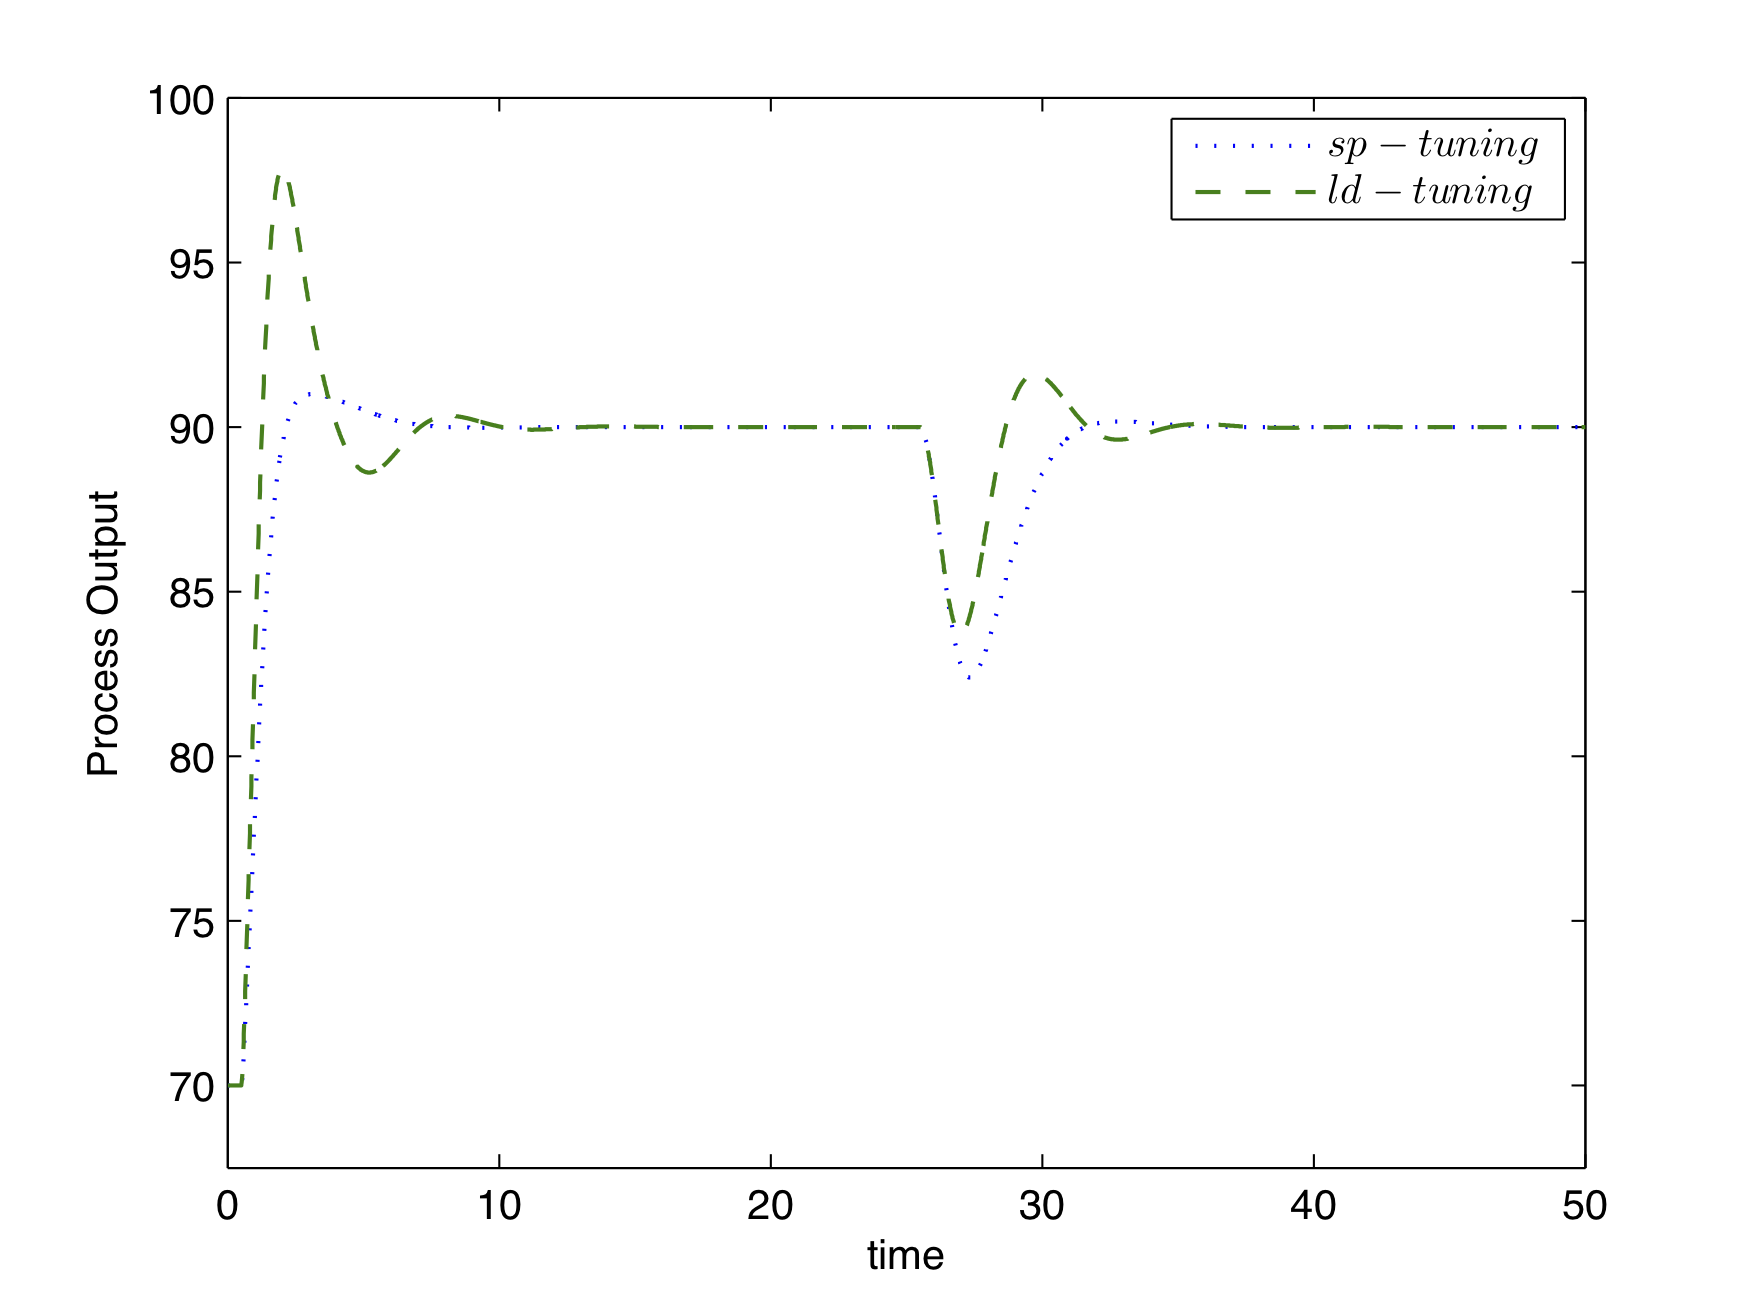
\includegraphics[width=\columnwidth]{Ch3fig22.png}
        \caption{Process responses for servo and regulation for system \eqref{system_example}.}
        \label{ch3:fig:example1}
    \end{center}
\end{figure}
%
%
\subsection{Performance vs. Robustness}
%
Robustness is an important attribute for control systems, because the design procedures are usually based on the use of low-order linear models identified at the closed-loop operation point. If only the system performance is taken into account, using for example an integrated error criteria (\gls{iae}, \gls{itae} or \gls{ise}), or a time response characteristic (overshoot, rise-time or settling-time for example), as was the case in \citet{Huang2002, Tavakoli2003}, the resulting closed-loop control system will probably have very poor robustness.

On the other hand, if the system is designed to have good robustness, as in \citet{Hagglund2008}, and if the performance of the resulting system is not evaluated, the designer will not have any indication of the \emph{cost} of having such a highly robust system.  System performance and robustness were take into account in \citet{Shen2002, Tavakoli2005}, optimizing its \gls{iae} or \gls{itae} performance but guarantying only the minimum accepted level of robustness ($M_S=2$). Therefore, the design of the closed-loop control system must take into account the system performance and its robustness, preserving the well-known \emph{trade-off} between all these variables.

At this point, we can revisit the \gls{cstr} reactor example from Chapter~\ref{chap:IndustrialPID}. In order to illustrate the performance/robustness trade-off, we apply the Model Reference Robust Tuning (MoReRT) method in order to tune a \gls{pid} controller for different levels of robustness \citep{Alfaro2016}.

As the MoReRT allows a desired robustness level to be imposed as a design specification, two cases have been considered here:
\begin{itemize}
	\item (a) for $M_S=2.0$, the controller parameters are: $K_p=3.335$, $T_i =0.685$~min, $T_d=0.181$~min,
	\item (b) for $M_S=1.6$, the controller parameters are: $K_p=2.372$, $T_i=0.663$~min, $T_d=0.162$~min.
\end{itemize}

 As can be seen, robust designs corresponding to lower values of $M_S$, yield lower controller gains. Consequently, time responses will be smoother but the performance indexes will worsen. Results are shown in Table~\ref{tab:cstrtradeoff} and Figure~\ref{ch3:fig:Ch3FigureClosedLoopRobustnessServoRegulation}. 
%
\begin{figure}[tb]
    \begin{center}
        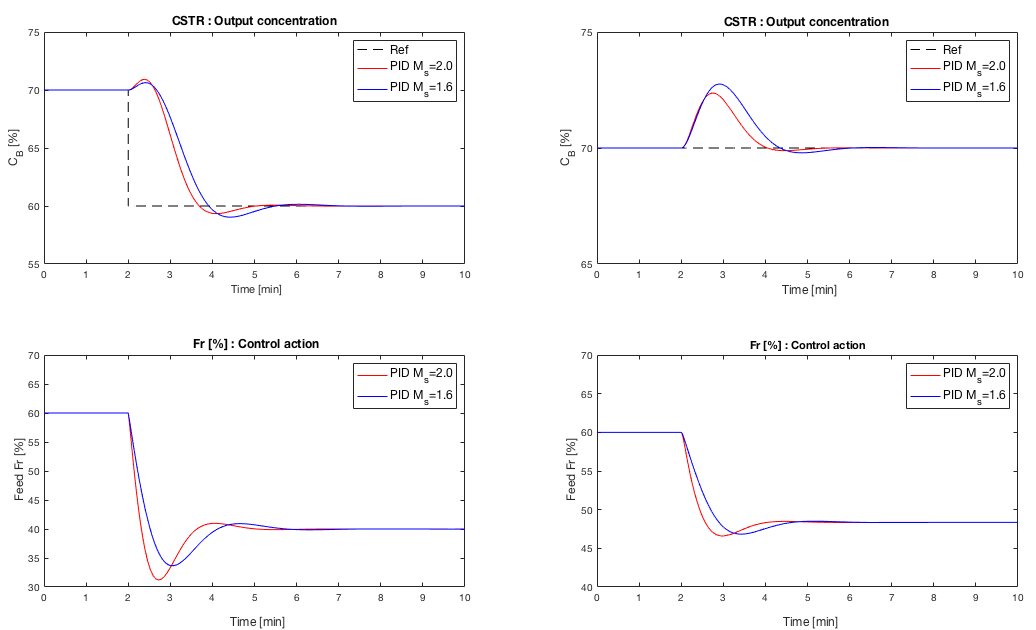
\includegraphics[width=\linewidth]{Ch3FigureClosedLoopRobustnessServoRegulation.png}
        \caption{CSTR reactor time output and control effort to a reference step change and disturbance at the inlet $C_{Ai}$ concentration }
        \label{ch3:fig:Ch3FigureClosedLoopRobustnessServoRegulation}
    \end{center}
\end{figure}

Table~\ref{tab:cstrtradeoff} shows the \gls{iae} performance indexes for the output concentration deviations as well as the \gls{tv} for the control effort corresponding to a disturbance change at the input concentration $C_{Ai}$ as well as to a desired change in the operating point, this is the desired output concentration $C_B$. We can conclude that the performance is worse for the more robust design but, on the other hand, the control effort becomes smoother. 
\begin{table}[tb]
	\caption{Robustness - Performance trade-off CSTR example} \label{tab:cstrtradeoff}
	\centering
    \begin{tabular}{ccccc}
    \toprule
    	 & \multicolumn{2}{c}{Set-point change for $C_B$}  & \multicolumn{2}{c}{Disturbance at $C_{Ai}$ concentration}\\
   		 & IAE & TV & IAE & TV\\
    \midrule
    $M_s=2.0$ PID Design   & 12.00 & 35.42 & 2.58 & 15.36 \\
    $M_s=1.6$ PID Design   & 14.05 & 34.30 & 3.66 & 13.60 \\
    \bottomrule
    \end{tabular}
\end{table}
%
\subsection{Input vs. Output Disturbances}
%
Disturbance attenuation is often recognized as the primary concern of a control system. Regulation of the operating conditions is the usual task to be pursued by a feedback controller. However, much of the academic works almost concentrate on set-point experiments for controller evaluation. Therefore, a controller design that emphasizes disturbance rejection rather than set-point tracking is an important design problem that, even if it has been the focus of research, may not have received the appropriate attention. Indeed much of the design approaches as well as application and/or simulation examples provided in academic works almost solely concentrate on set-point experiments for controller evaluation. Even those that explicitly focus on the disturbance attenuation problem, usually only concentrate on input load disturbances.

There is however a disturbance attenuation consideration not taken into account, as far as the knowledge of the author, which is of considering a different load disturbance dynamics path. As mentioned in \cite{Shinskey2002}, there are some processes that exhibit different dynamics in the load path. These include heat exchangers, where the load can enter the tube bundle whereas the manipulated flow enters the shell (or vice versa), and distillation columns, where the load is the feed and the manipulated variables are the reboiler flow rate and the reflux.

As a matter of a simple example, the controller used in the previous section, the one with $M_S=2.0$ is faced here against three different disturbances:
%
\begin{itemize}
\item A load disturbance, which is one that enters at the process input. This is exemplified here by a 10\% disturbance at the inlet flow rate $F_r$.
\item A disturbance that enters at an intermediate point of the process dynamics. This is exemplified here by a 10\% disturbance at the inlet concentration of the $A$ component.
\item A disturbance that affects directly at the process output. This is exemplified here by a 10\% disturbance at the output concentration of the $B$ component $C_B$.
 \end{itemize} 

As can be seen in Figure~\ref{ch3:fig:Ch3FigureClosedLoopDisturbances}, even if the size of the disturbance is the same in all three situations, the response of the controller is different. In the case of the output disturbance response, its dynamics are similar to the one for a reference change (not shown in the figure). In fact, the disturbance signal enters at the same point in the block diagram (except for eventual sensor measurement noise).

Therefore, depending on the control system specifications, the attenuation of one disturbance or the other requires different considerations. This means that, in addition to the other two trade-offs just presented above (servo an load regulations responses), a third potential source of conflicting objectives motivates the need for a multiobjective approach.
%
\begin{figure}[tb]
    \begin{center}
        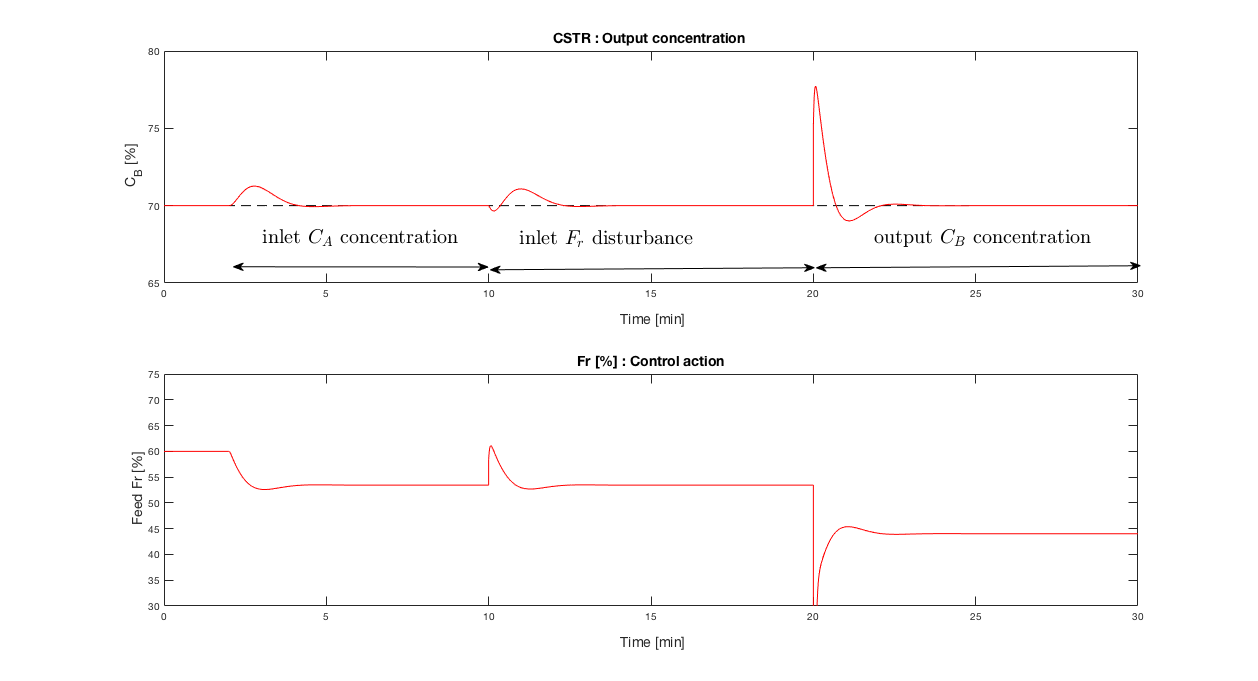
\includegraphics[width=\columnwidth]{Ch3FigureClosedLoopDisturbances.png}
        \caption{CSTR output $C_B$ concentration in response to different disturbances.}
        \label{ch3:fig:Ch3FigureClosedLoopDisturbances}
    \end{center}
\end{figure}
%
\bibliographystyle{spbasic}
\bibliography{ReferenciasMulti}